
\subsection{Tightly Coupled HPC Workloads} 
\label{tcp_hpc_workloads}

As described in section \ref{state_of_the_art_tcp} \ac{TCP} problems are a large part of the \ac{HPC} world,  but seem to lack native support in Pachyderm.
Pachyderm as it exists as of writing this thesis, is centralized around \ac{LCP} problems, as it is designed to work with large amounts of data but with each so called "datum" being independent of each other.
This is a very good fit for \ac{LCP} problems, and ties into their concepts of data lineage, versioning and providence.

\begin{figure}[htb]
    \centering
    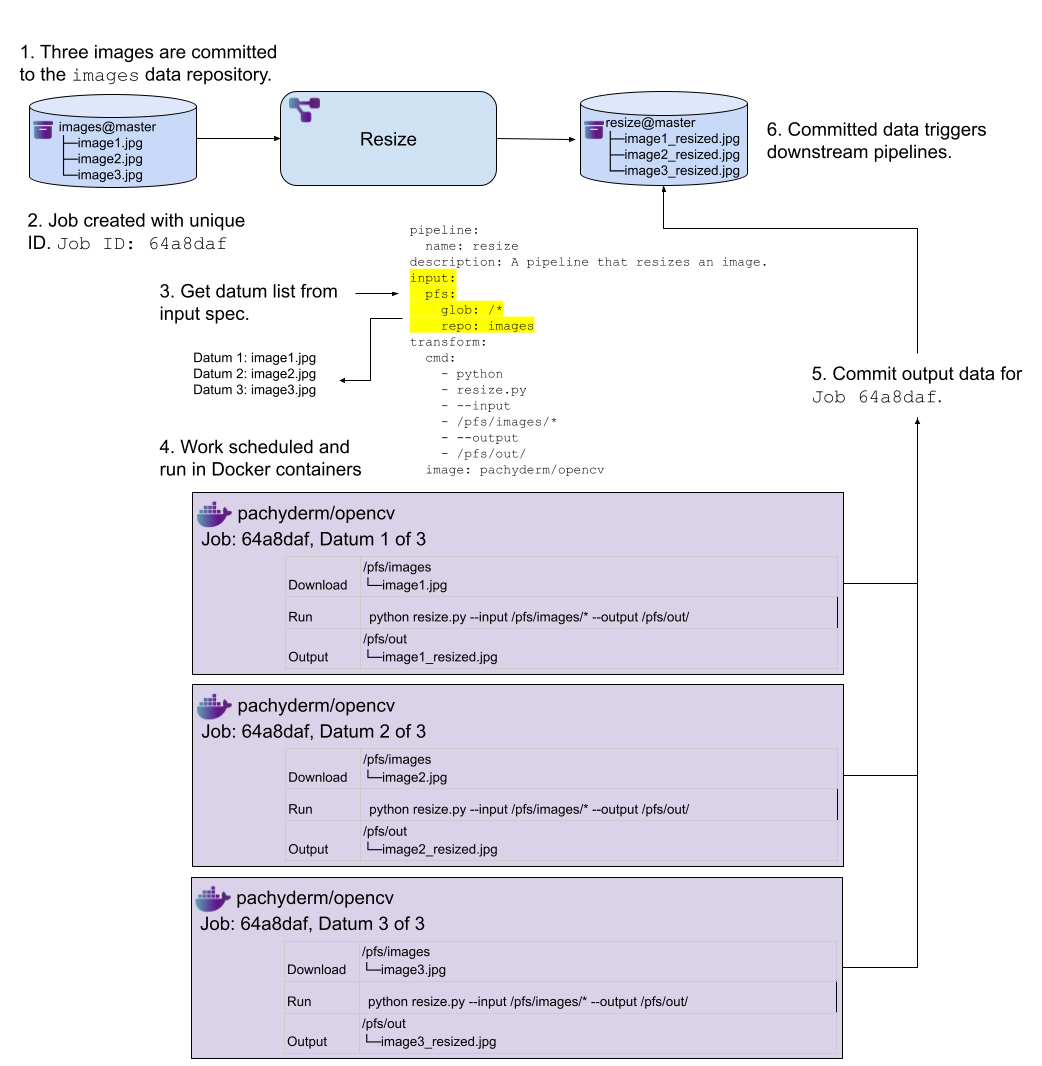
\includegraphics[width=14cm]{graphics/datum_distribution_amongst workers.png}
    \caption[Pachykouda datum distribution amongst workers]{Pachykouda datum distribution amongst workers \footnotemark}
    \label{abb:datum_distribution_amongst workers}
\end{figure}
\footnotetext{Taken from: \cite{IntroPipelines2023}}


Diagram \ref{abb:datum_distribution_amongst workers} shows Pachyderms approach to distribute their datums amongst workers, given an already defined pipeline.
Once Data files are added to the input repository, Pachyderm will determine Based on a glob pattern wether the files are relevant datums for the pipeline.
If the newly added data fits the pattern each of the files will be supplied to its own instantiation of a worker, all originating from the same image, which will then process the data concurrently and independently of each other.
After the worker has finished its task, the resulting datums are then collected in their own repository of data.
A more detailed swim lane diagram of this process can be found in the appendix at \ref{abb:pipeline_communication_sld}

This approach is very well suited for \ac{LCP} problems, as the datums are independent of each other and can be processed in parallel without any issues.
But it is not well suited for Large \ac{TCP} problems, if the computation of the data can not be split into distinct independent datum files, or the computation is reliant on the intercommunication of the datums.
If the datasets are small enough, this does not really present a problem as one can simply take all the data into a single worker node and process it there.
But as a single worker node can only utilize the resources of a single physical compute node, this does not scale well with the size of the dataset and defeats the purpose of a distributed system in the first place.

So our goal for this section is a way to find a way to enable pachyderm to pool the entire resources of the cluster, in order to solve a \ac{TCP} problem.

\subsubsection{First iteration - PachyKouda}

As a first attempt to address this issue, it was decided that the integration of a \ac{TCP} framework into Pachyderm on the container level would be the best approach.
So the first iteration is based on the idea of a Pachyderm conforming client container, which is able to interface with an external \ac{TCP} framework,
which can handle the reception of the data, the distribution of the data amongst the workers and the collection of the results to reintegrate them into the \ac{PFS}.

The first iteration of this idea was called PachyKouda, as it was based on the Arkouda \ac{TCP} framework\footcite{ArkoudaGituhbRepository2023},
which itself is a python binding for the Chapel programming language \footcite{ChapellangChapelProductive}. 

For that step an Arkouda worker was installed bare metal on the head node of the Heydar cluster, in order to verify the feasibility of the idea,
with the goal of moving the worker into the cluster in the next iteration.

The client container was based on the official \ac{UDP}-based build by the Arkouda team \footcite{ArkoudacontribArkoudadockerMain}.
The container was then modified to be able to communicate with the Arkouda worker on the head node of the cluster, it can now send data to the worker and receive the results.

\subsubsection*{Learnings from the first iteration}

The first iteration was a total success, as it proved the feasibility of being able to use a client container to forward the data processing to an external Arkouda worker.
As described earlier, the goal of the next iteration is to move the Arkouda worker into the cluster, in order to be able to utilize the full resources of the cluster.

\subsubsection{Second iteration - Kymera}

\begin{figure}[htb]
    \centering
    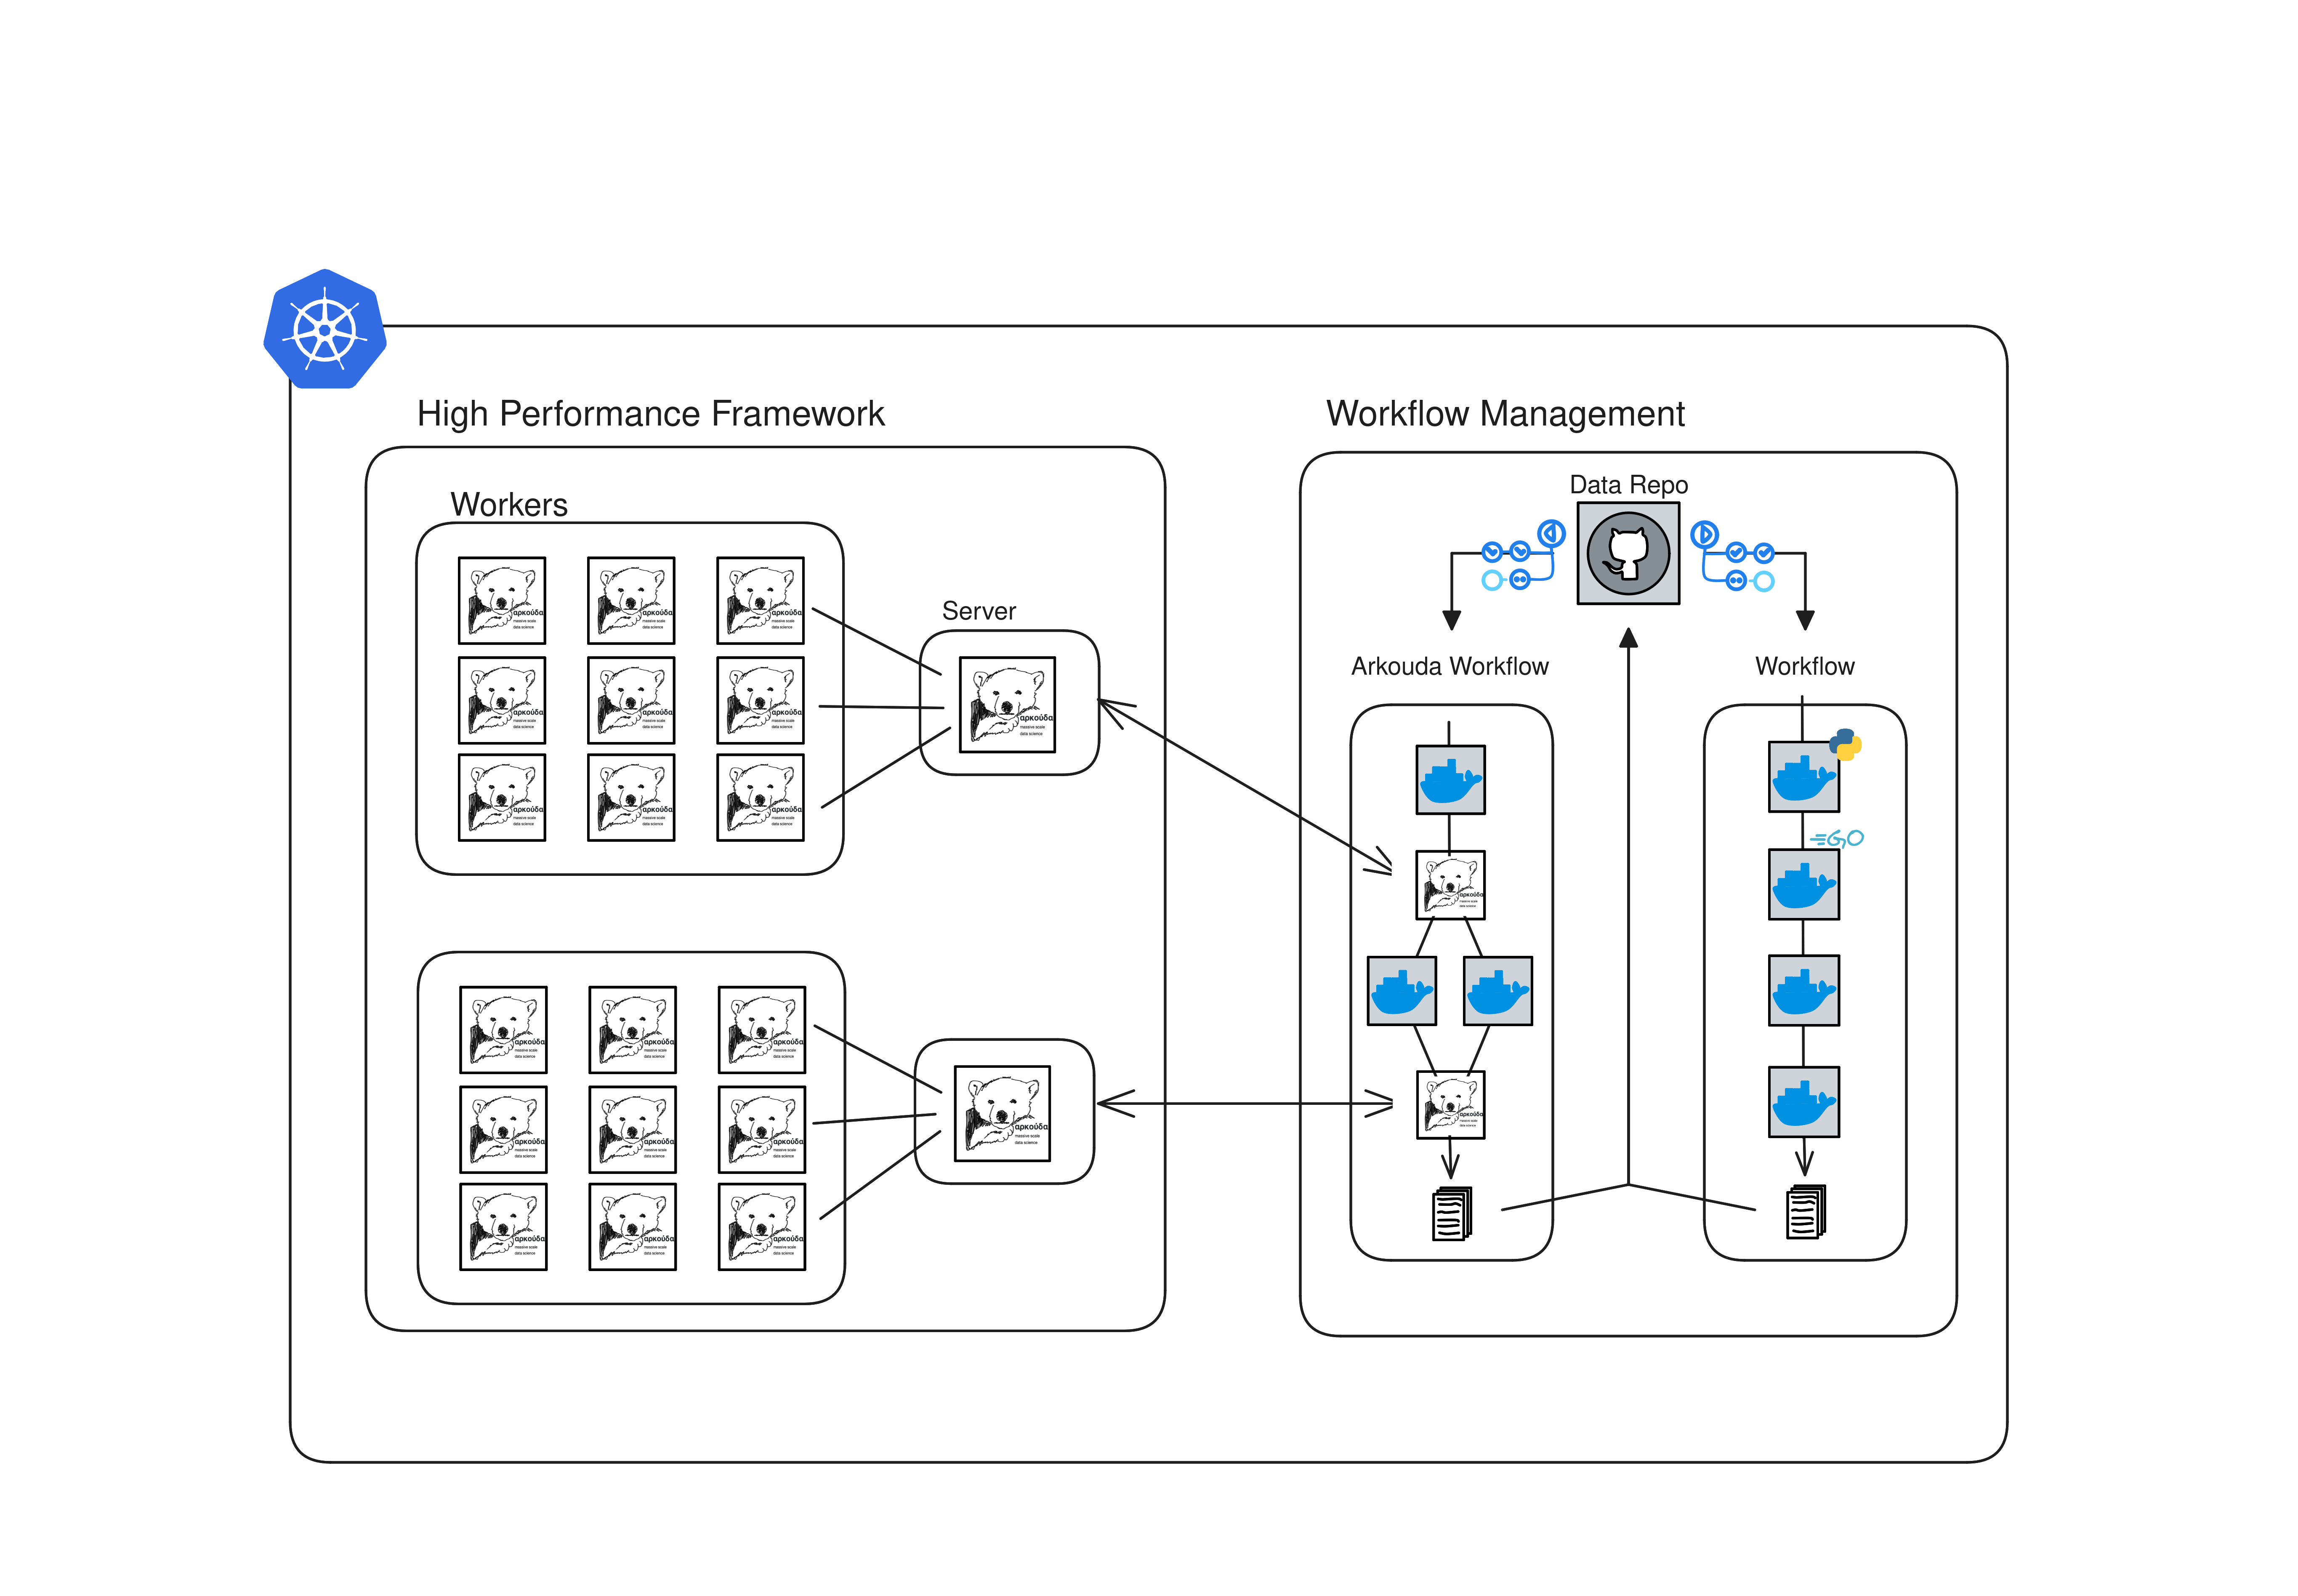
\includegraphics[width=16cm]{graphics/PachyKouda.png}
    \caption[Arkouda workers on \ac{k8s}]{Arkouda workers on the Heydar cluster}
    \label{abb:arkouda_workers_on_k8s}
\end{figure}

Diagram \ref{abb:arkouda_workers_on_k8s} above shows a high level overview of how the workers interface with the client container in the workflow.
The Arkouda container which is part of the workflow is still the same as in the first iteration, but now instead of interfacing with an external worker it 
is interfacing with a worker swarm hosted across the cluster.

The Swarm is split into two parts, one central Arkouda server, facilitating the communication between the client container and the workers and the workers also called locales themselves.
The locales and the server are based on the helm charts provided by the Arkouda-Contrip repo\footcite{BearsRUsArkoudacontribArkoudahelmcharts},

A detailed walk through the setup of the \ac{RBAC}, Secrets and deployments for the Heydar Cluster can be found in the project repo\footcite{HeydarSetup} which in turn is based on the official
Arkouda documentation\footcite{ArkoudacontribArkoudadockerMain}.

\subsubsection*{Learnings from the second iteration}
As Arkouda does not currently provide multi tenancy of their Server, meaning that they can only be connected a single client at a time, 
so if multiple pipelines need to solve a \ac{TCP} at the same time, they would not be able to share the same worker swarm.
Instead, they would need to spawn their own worker swarm.

Another issue is that there are currently going through the standard Pod to pod communication configuration of flannel, which means that the entire traffic between the client container and the Arkouda server 
as well as the traffic between the workers is all happening over emulated overlay network which enables the containers on the different nodes to communicate with each other as if they where on the same network, no matter of the actually infrastructure below it.
The communication protocol of the Arkouda servers is \ac{UDP} based \ac{GASNet}, which provides the \ac{RDMA} needed for the Arkouda framework to work, but this incurs a significant overhead in the form of the encapsulation of the \ac{UDP} packets into \ac{TCP} packets.

Also, the containers are currently not compatible with the OpenFAM project \footcite{keetonOpenFAMAPIProgramming2019}, which is being developed as an integration to Arkouda and Chapel by the Hewlett Packard Systems Architecture Lab \footcite{byrneCouplingChapelPoweredHPC2023},
it extends the Arkouda framework with the ability to use \ac{FAM} as banks of \ac{RDMA} enabled memory, which can be accessed by the Arkouda workers.
This would proof to be a significant improvement as it has the potential to reduce the overall overhead of the communication\Footcite{chouOptimizingPostCopyLive2019} amongst the workers as well as to the server, by cutting down the overall amount of network traffic.

The pachyderm platform itself might also benefit from the integration of \ac{FAM}, as it could be used to store the datums in the \ac{PFS}, providing the running pipeline processes with a much faster access to the data.

\subsubsection{Third iteration - \ac{FAM}}
\label{third_iteration_fam}
While significant efforts have already been made to successfully integrate Arkouda and \ac{FAM}, these have so far been focussing on bare metal installations, for that reason, in order to integrate the \ac{FAM} enabled Arkouda working from within a containerized environment the tools would need to be 
custom recompiled matching the new environment. 
Therefore, we needed to:

\begin{enumerate}
    \item Compile OpenFAM in the Container
    \item Compile custom Chapel in the Container with OpenFAM
    \item Compile custom Arkouda in the Container with the OpenFAM enabled Chapel
    \item Rebuild the Arkouda container with the new Arkouda binary
    \item Reweite the \ac{k8s} deployment to make use of OpenFAM
\end{enumerate}

This section was quite challenging as it required a deep understanding of the \ac{PoC} implementations of the OpenFAM, Arkouda and Chapel projects and was cut short by the time constraints of the project and was therefore not brought to a successful conclusion.
\textcolor{red}{The current state of the project can be found in the \ac{PoC} repository\footcite{eckerthPoCRepository2023} and in the appendix at \ref{appendix:arkouda_fam}. 
}
But this showed us that there is a lot of potential in the integration of \ac{FAM} into the container based \ac{HPC} world, as it could provide a significant performance boost to the overall system and should be explored further in future iterations.

